% generated by experiments/build_paper_assets.py -- do not edit by hand
\begin{figure}[t]
\centering
\resizebox{\linewidth}{!}{%
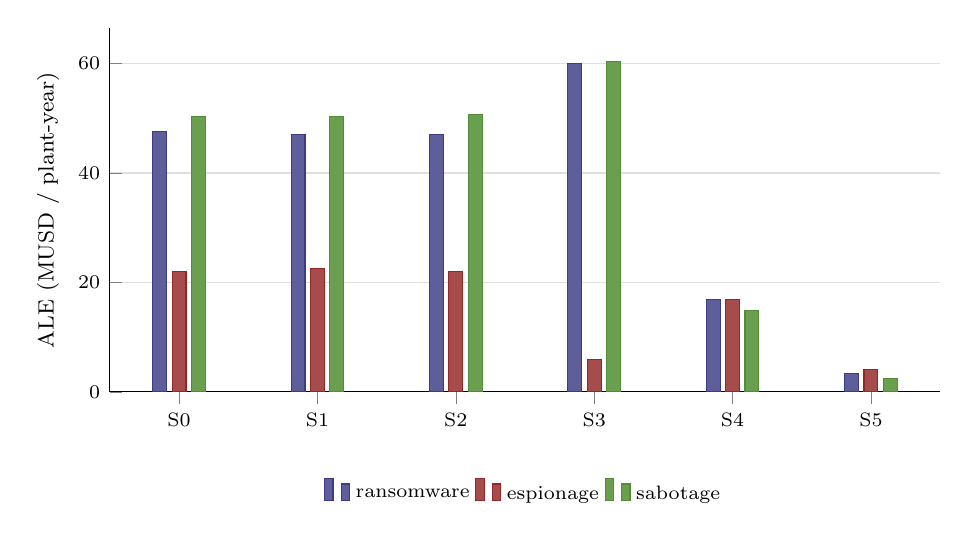
\begin{tikzpicture}
\begin{axis}[
    ybar, width=\linewidth, height=6.2cm,
    ylabel={ALE (MUSD / plant-year)},
    symbolic x coords={S0,S1,S2,S3,S4,S5}, xtick=data,
    ymin=0, bar width=5pt, enlarge x limits=0.10,
    legend style={at={(0.5,-0.22)}, anchor=north, legend columns=3, font=\scriptsize,
                   draw=none},
    ticklabel style={font=\scriptsize}, label style={font=\footnotesize},
    ymajorgrids, grid style={gray!25}, axis lines*=left,
]
\addplot[fill=MidnightBlue!70, draw=MidnightBlue!85] coordinates {(S0,47.57) (S1,47.0) (S2,47.01) (S3,60.09) (S4,16.86) (S5,3.37)};
\addplot[fill=Maroon!70, draw=Maroon!85] coordinates {(S0,21.97) (S1,22.49) (S2,22.04) (S3,5.92) (S4,16.94) (S5,4.13)};
\addplot[fill=OliveGreen!70, draw=OliveGreen!85] coordinates {(S0,50.41) (S1,50.38) (S2,50.71) (S3,60.42) (S4,14.93) (S5,2.46)};
\legend{ransomware, espionage, sabotage}
\end{axis}
\end{tikzpicture}}
\caption{Annualised loss expectancy per control scenario and actor profile. Scenario $S_3$ lowers espionage risk sharply while \emph{increasing} ransomware risk: hardening the cheap data-theft routes displaces a rational actor onto the availability objective.}
\label{fig:scenario-ale}
\end{figure}
